\shorthandoff{"}
\chapter{Person-Environment Fit}
\label{ch:personEnvironmentFit}

\section{Einführung}
\label{ch:personEnvironmentFit:einfuehrung}
Der Person-Environment Fit ist ein Konzept in der Organisationspsychologie \cite[S. 1f.]{edwards:2008}. Er enthält drei zentrale Größen: Person, Umgebung (Environment) und Ergebnis (Outcome) \cite[S. 2f.]{livingstone:1997}. Forscher dieses Fachgebietes gehen davon aus, dass ein Ergebnis stets vom Zusammenspiel von Person und Umgebung abhängig ist und nicht durch eine der beiden Größen alleine bestimmt wird \cite[S. 1]{muchinsky:1987}.\\
\textcite[S. 5]{edwards:2007} stellen fest, dass die Literatur unter der Person meist ein menschliches Individuum versteht. Umgebung und Ergebnis interpretieren verschiedene Publikation ihren Beobachtungen zu Folge dagegen als breite Terminologien. Diese werden je nach Forschungsdomäne genauer spezifiziert. Beispiele für Ergebnisse sind Zufriedenheit \cite[S. 1]{lashani:2021}, Wechselbereitschaft \cite[S. 1]{amarneh:2021}, Kreativität \cite[S. 1]{duan:2019}, Leistung \cite[S. 7f.]{elfenbein:2007} und  Berufswahl \cite[S. 1]{cable:1996}. Als Umgebung untersuchten verschiedene Publikationen unter anderem Unternehmen \cite[S. 1]{kristof:1996}, Gruppen \cite[S. 1]{werbel:2001} und Arbeitsplätze \cite[S. 1]{lu:2014}.\\
Der Person-Environment Fit gibt an, zu welchem Grad sich die untersuchten Werte von Person und Umgebung auf einem Niveau befinden \cite[S. 3]{chatman:1989}. Wie in Abbildung \ref{fig:personEnvironmentFit:einfuehrung:abb1} verdeutlicht, ist der Fit selbst kein Ergebnis, sondern eine unabhängige Variable, welche zur Bestimmung eines untersuchten Resultates herangezogen wird \cite[S. 4f.]{edwards:1991}.\\
\begin{figure}[h]
	\centering
	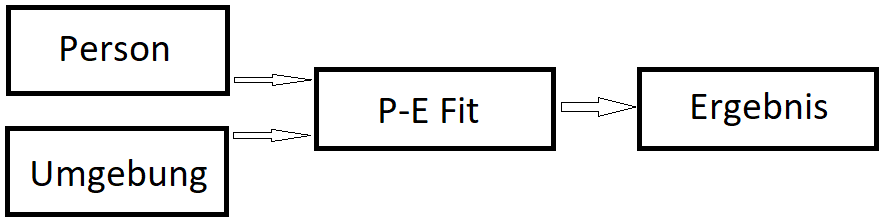
\includegraphics[width=1\textwidth]{gfx/P-E Fit.png}
	\caption{Nochmal schön machen und kennzeichnen, dass die P-E-Beziehung wechselseitig ist}
	\label{fig:personEnvironmentFit:einfuehrung:abb1}
\end{figure}\\
Der Person-Environment Fit wird auch als P-E Fit abgekürzt \cite[S. 428]{dawis:2002} und findet sich in verschiedenen Publikationen ebenfalls unter ähnlichen Bezeichnungen mit derselben Bedeutung wie Match \cite[S. 2]{player:2017}, Korrespondenz \cite[S. 1]{eggerth:2008} oder Kongruenz \cite[S. 1]{muchinsky:1987}. In der Literatur wird der P-E Fit nicht als Zustand, sondern als wechselseitiger Prozess betrachtet. In diesem interagieren Person und Umgebung miteinander und verändern sich dabei gegenseitig \cite[S. 21f.]{roberts:2006}. Diese Modifikationen können die Kongruenz sowohl verbessern als auch verschlechtern \cite[S. 4]{caplan:1987}. Aus diesem Grund wurden in der Literatur auch Maßnahmen erforscht, welche den Person-Environment Fit gezielt optimieren sollen \cite[S. 16]{cable:2001}.\\
Wie die Kongruenz von Person und Umgebung berechnet wird, ist von der konkreten Art des Fits abhängig. \textcite[S. 1]{muchinsky:1987} unterscheiden dabei zwischen ergänzendem (supplementary) und komplementären (complementary) Fit.

\section{Ergänzender und komplementärer Fit}
\label{ch:personEnvironmentFit:supplementaryUndComplementary}
Ein ergänzender Fit entsteht, wenn Person und Umgebung gleiche Werte und Interessen aufweisen \cite[S. 2f.]{muchinsky:1987}. Diese Art von Kongruenz ist laut \textcite[S. 1ff.]{schneider:1987} ein entscheidender Faktor, von welchen Unternehmen sich potentielle Arbeitnehmer angezogen fühlen und welche Bewerber von Betrieben eingestellt werden. Auch \textcite[S. 7]{devendorf:2008} stellten fest, dass sich potentielle Arbeitnehmer stärker zu Unternehmen angezogen fühlen, bei deren Mitarbeitern sie eine hohe Ähnlichkeit zu sich selbst wahrnehmen. \textcite[S. 4]{popovich:1982} zu Folge kann der Beitritt einer Person zu einem Unternehmen sogar als ein "sehr konkreter, öffentlicher Ausdruck der Werte"\footnote{"a very concrete, public expression of values" - \textcite[S. 4]{popovich:1982}} eines Individuums interpretiert werden.\\
Verschiedene Autoren diskutieren die Ergebnisse des ergänzenden Fits in der Literatur kontrovers. \textcite[S. 6]{schneider:1987} stellte fest, dass Angestellte mit einer geringen Werte-Übereinstimmung eher dazu tendieren, ihr Unternehmen zu verlassen. So entsteht im Betrieb langfristig eine hohe Homogenität innerhalb der Belegschaft. Diese äußert sich einerseits in positiven Ergebnissen wie einer ausgeprägten Arbeitszufriedenheit, geringer Wechselbereitschaft und starker Identifikation mit dem Unternehmen \cite[S. 25ff.]{kristof:1996}\cite[S. 5]{su:2015}. Die mangelnde Diversität führt aber anderseits auch zu negativen Folgen, wie einer geringeren Bereitschaft für Veränderungen \cite[S. 10]{schneider:1987} und verminderter Kreativität und Innovation im Unternehmen \cite[S. 7]{chatman:1998}.\\
Wenn sich Person und Umgebung nicht ähneln, sondern gegenseitig vervollständigen, sprechen \textcite[S. 4]{muchinsky:1987} vom komplementären Fit. Dabei gleichen Person und Umgebung den Autoren zu Folge Schwächen des anderen durch eigene Stärken aus.\\
Die komplementäre Kongruenz wird wie in Abbildung \ref{fig:personEnvironmentFit:supplementaryUndComplementary:abb1} dargestellt, in zwei weitere Fits untergliedert. Bei dieser Betrachtungsweise haben Person und Umgebung je eine Angebots- und eine Nachfrageperspektive. Die Nachfrage der einen Partei wird dabei durch das Angebot der anderen erfüllt \cite[S. 2ff.]{caplan:1987}\cite[S. 2f.]{edwards:1991}.\\
\begin{figure}[h]
	\centering
	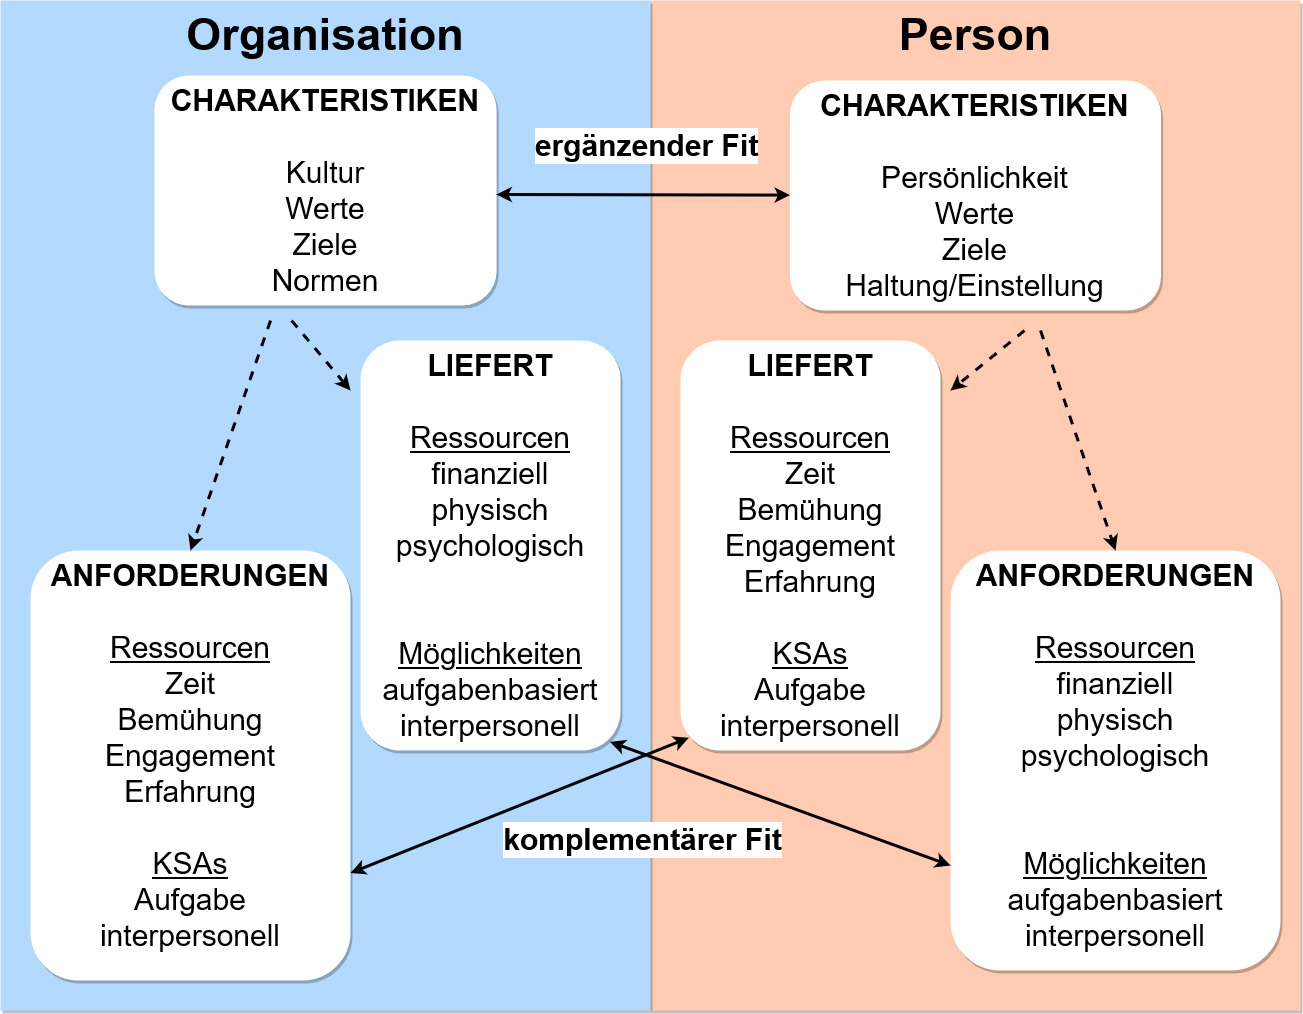
\includegraphics[width=1\textwidth]{gfx/supplementaryComplementaryFit.png}
	\caption{Hier eine Beschreibung einfügen; Quelle: \cite[S. 4]{kristof:1996}}
	\label{fig:personEnvironmentFit:supplementaryUndComplementary:abb1}
\end{figure}
\\
Unter der Nachfrage der Umgebung werden die in Abbildung \ref{fig:personEnvironmentFit:supplementaryUndComplementary:abb1} dargestellten Anforderungen (Demands) an die Person zusammengefasst. Hierzu zählen beispielsweise Rollen- und Leistungserwartungen. Das entsprechende Angebot der Person sind ihre Fähigkeiten (Abilities). Diese umfassen unter anderem Fertigkeiten, Wissen, Bildung und Arbeitserfahrung. Befinden sich Nachfrage der Umgebung und Angebot der Person auf einem Niveau, entsteht der Anforderungen-Fähigkeiten Fit (Demands-Abilities Fit). Dieser resultiert in einer hohen Leistung und Effizienz der Organisation \cite[S. 3f.]{edwards:1991}\cite[S. 5]{edwards:1996}\cite[S. 4f.]{edwards:2007}\cite[S. 6]{su:2015}.\\
Die Nachfrage der Person entspricht ihren psychologischen Bedürfnissen (Needs). Dazu zählen persönliche Präferenzen, Interessen, Motive und Ziele. Die entsprechenden Angebote (Supplies) der Umgebung umfassen Ressourcen und Belohnungen wie Gehalt und Mitbestimmungsrechte, welche die Bedürfnisse des Individuums befriedigen. Sind Nachfrage der Person und Angebote der Umgebung gleich stark ausgeprägt, wird dies in der Literatur als Bedürfnisse-Angebote Fit (Needs-Supplies Fit) bezeichnet. Dieser resultiert in einem hohen Wohlbefinden des Mitarbeiters, welches sich beispielsweise in Zufriedenheit und verminderter Wechselbereitschaft äußert \cite[S. 2]{edwards:2004}\cite[S. 2f.]{edwards:1996}\cite[S. 4]{edwards:2008}\cite[S. 4f.]{edwards:2007}\cite[S. 6]{su:2015}.\\
Laut \textcite[S. 9ff.]{workAdjustment:1964} und \textcite{wanous:1992} führen unausgeglichene Charakteristiken auch beim komplementären Fit langfristig zu einem Wechsel des Arbeitsplatzes. Die Autoren betrachten die aus einem unzureichenden Anforderungen-Fähigkeiten Fit entstehende mangelnde Arbeitsleistung als Ursache für Kündigung oder Versetzung des Mitarbeiters seitens des Unternehmens. Die aus einem Fähigkeiten-Angebote Ungleichgewicht resultierende Unzufriedenheit ist dagegen ein Wechselgrund seitens des Mitarbeiters.\\
\textcite[S. 1ff.]{edwards:2004} bezeichnen ergänzende und komplementäre Kongruenz als unterschiedliche, parallele Strömungen innerhalb der P-E Fit-Forschung. Doch sie stellen fest, dass beide Fits nicht vollkommen unabhängig voneinander sind. Die Ursache sehen sie in den inneren Werten von Person und Umgebung. Diese sind einerseits ausschlaggebend für den ergänzenden Fit, beeinflussen aber auch stark die Bedürfnisse der Person und die Angebote der Umgebung. So würde sich ein Individuum mit ausgeprägten familiären Werten aufgrund des ergänzenden Fits stark zu Betrieben mit denselben Eigenschaften angezogen fühlen. Gleichzeitig prägt die Person aufgrund ihrer inneren Werte im komplementären Fit das Bedürfnis nach familiären Reizen wie gemeinschaftlichen Veranstaltungen aus. Da das Unternehmen dieselben Eigenschaften besitzt, wird dieses seinen Mitarbeitern die Teilnahme an derartige Ereignisse anbieten.\\
Dass der Abgleich der Charakteristiken von Person und Umgebung sehr bedeutsam für Zufriedenheit und Produktivität sind, erkannten Psychologen bereits vor über einhundert Jahren \cite[S. 5ff.]{parsons:1909}. Die Wurzeln des Person-Environment Fits reichen zurück bis ins Jahr 1909 \cite[S. 1]{su:2015}.

\section{Historische Entwicklung}
\label{ch:personEnvironmentFit:historisches}
Im ersten Jahrzehnt des 20. Jahrhunderts beschäftigten sich Wissenschaftler und Psychologen in zahlreichen Ländern der westlichen Welt intensiv mit dem Thema der Personalauswahl \cite[S. 1]{salgado:2001}. Ein Hauptanliegen der Forscher war es, individuelle Unterschiede zwischen den Menschen anzuerkennen und bei der Berufswahl zu berücksichtigen \cite[S. 2ff.]{stern:1900}. Deren Ansichten zu Folge würde die gesamte Gesellschaft effizienter arbeiten, wenn Menschen eine zu ihren wissenschaftlich ermittelten Fähigkeiten passende Tätigkeit aufnehmen würden \cite[S.2]{kevles:1968}\cite[S. 3]{parsons:1909}. Im Zuge dieser Entwicklungen konzipierte der Bostoner Professor Frank Parsons eine Vorgehensweise zur Berufsfindung, welche im Jahr 1909 vorgestellt wurde \cite[S. 1]{su:2015}. \textcite[S. 5ff.]{parsons:1909} erkannte schon zum damaligen Zeitpunkt, dass das Gleichgewicht von eigenen Fähigkeiten und Anforderungen des Berufsumfeldes eine wichtige Ursache für Effizienz, Produktqualität und Bezahlung waren. Aus diesem Grund empfahl er jungen Menschen vor der Berufswahl zunächst ihre eigenen Fähigkeiten, die Anforderungen verschiedener Arbeitsplätze und die Beziehung zwischen beiden Seiten zu verstehen. Erst wenn eine Person diese Punkte unter Beaufsichtigung eines Berufsberaters und durch Verwendung verschiedener wissenschaftlicher Tests erfüllt, könne sie sich für einen passenden Beruf entscheiden. Heute gilt Parsons aufgrund dieser Gedanken als "Gründungsvater der Berufsberatung"\footnote{"founding father of vocational guidance" - \textcite[S. 3]{porfeli:2009}} \cite[S. 3]{porfeli:2009} und als erster Vorläufer des Person-Environment Fits \cite[S. 2]{edwards:2008}.\\
Zum damaligen Zeitpunkt begegnete die Bevölkerung psychologischen Tests zunächst mit Skepsis \cite[S. 2]{kevles:1968}. Das änderte sich im Jahr 1917 mit dem Eintritt der Vereinigten Staaten in den Ersten Weltkrieg. Das U.S. Militär stand vor der Herausforderung, innerhalb kürzester Zeit Millionen Männer in die verschiedenen spezialisierten Rollen des technisierten Krieges einzuordnen. Zu diesem Anlass setzten Wissenschaftler erstmals im großen Stil psychologische Tests zur Zuweisung von Personen zu passenden Militärpositionen ein \cite[S. 2ff.]{kevles:1968}. \\
Nach dem Ersten Weltkrieg entstanden insbesondere in den 1930er-Jahren durch die Arbeiten von Lewin und Murray weitere bedeutende Entwicklungen für die Entstehung des Person-Environment Fits \cite[S. 1]{edwards:1990}. \textcite[S. 11f.]{lewin:1936} stellte fest, dass das Verhalten eines Menschen nicht, wie bis dahin angenommen, nur durch das Individuum selbst, sondern durch das Zusammenspiel von Person und Umgebung zu erklären ist. Aufbauend auf diesen Erkenntnissen erarbeitete \textcite[S. 38ff.]{murray:1938} sein Need-Press-Modell. Der Wissenschaftler ging davon aus, dass jeder Mensch im Laufe seines Lebens verschiedene Bedürfnisse (Needs) unterschiedlich stark ausprägt. Diese treffen in verschiedenen Umgebungen auf diverse Reize. Murray stellte fest, dass manche Reize mit bestimmten Bedürfnissen kompatibel sind. Trifft ein passendes Bedürfnis-Reiz-Paar aufeinander, entsteht Druck (Press). Personen interpretieren diesen subjektiv als schädliche oder nützliche Situation und zeigen eine entsprechende Reaktion. Dieses Zusammenspiel von Bedürfnissen einer Person und Reizen der Umgebung entspricht der späteren Vorstellung des Bedürfnisse-Angebote Fits \cite[S. 8]{edwards:2008}. \\
Die Erkenntnisse von Lewin und Murray gelten als wichtiger Grundstein für die Arbeiten verschiedener Forschungsgruppen rund um John R. P. French, Jr. \cite[S. 5]{caplan:1993}. Der Psychologe stellte im Jahr 1963 an der Universität in Michigan ein groß angelegtes Forschungsprogramm vor. Dieses machte es sich zum Ziel, die Auswirkungen des sozialen Umfeldes in Industrie-Unternehmen auf die Gesundheit der Mitarbeiter zu untersuchen. Zu diesem Zweck arbeiteten Experten verschiedener Fachrichtungen eng zusammen \cite[S. 1ff.]{french:1963}. Aus dieser Kollaboration entstand die erste formale Definition des Person-Environment Fits. Diese präsentierten \textcite{copingAndAdaption:1974} im Jahr 1974. Dabei unterschieden die Forscher ausgehend ihren bis dahin erzielten Erkenntnissen zwischen objektivem und subjektivem Fit \cite[S. 4f.]{caplan:1993}\cite[S. 1ff.]{french:1966}.

\section{Objektiver und subjektiver P-E Fit}
\label{ch:personEnvironmentFit:subjektivObjektiv}
% Hierzu Quellen von Caplan und Harrison einfügen, sobald Bücher verfügbar
\textcite{copingAndAdaption:1974} erforschten die Auswirkungen des Zusammenspiels von Individuum und Arbeitsumgebung auf die mentale Belastung des Mitarbeiters. Wie in Abbildung \ref{fig:personEnvironmentFit:subjektivObjektiv:abb1} dargestellt, gingen die Wissenschaftler davon aus, dass von Person und Umgebung je eine objektiv messbare und eine vom Mitarbeiter subjektiv wahrgenommene Version existieren. \\
\begin{figure}[h]
	\centering
	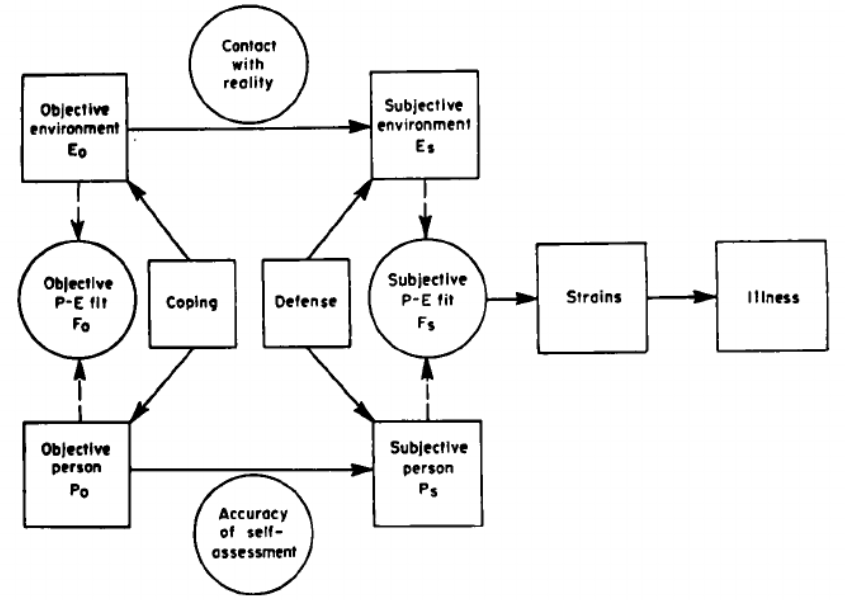
\includegraphics[width=1\textwidth]{gfx/subjektivObjektivPEFit.png}
	\caption{Hier eine Beschreibung einfügen \cite[S. 22]{edwards:2008}}
	\label{fig:personEnvironmentFit:subjektivObjektiv:abb1}
\end{figure}
\\
\textcite{copingAndAdaption:1974} betonten die Wichtigkeit, alle vier Subjekte anhand vergleichbarer Dimensionen zu messen. Dies betrachteten sie als wichtige Grundlage, um aussagekräftige Ähnlichkeiten berechnen zu können. In ihren Untersuchungen bestimmten sie die in Abbildung \ref{fig:personEnvironmentFit:subjektivObjektiv:abb1} dargestellten Differenzwerte des objektiven und des subjektiven P-E Fits.\\
Individuen streben den Wissenschaftlern zu Folge an, unerfüllte Anforderungen zu verhindern. Dies gilt sowohl für unbefriedigte Bedürfnisse der Person als auch für überhöhte Ansprüche der Umgebung. Um solche Situationen zu vermeiden, existieren zwei Strategien. Ändert ein Mitarbeiter seine objektive Umgebung oder sein objektiv ermitteltes Selbst zur Verbesserung des objektiven P-E fits, sprechen \textcite{copingAndAdaption:1974} von Bewältigung (Coping). Ändert die Person ihre subjektive Wahrnehmung von Umgebung oder sich selbst zur Optimierung des subjektiven P-E fits, bezeichnen sie die Strategie als Verteidigung (Defense). Beispielsweise könnte sich ein Bachelor-Absolvent für eine Stelle interessieren, welche als Anforderung einen Master-Abschluss voraussetzt. Diese Unterschiede im objektiven P-E Fit könnte die Person bewältigen, indem sie entweder den fehlenden Abschluss erwirbt oder das Unternehmen überzeugt, die Stellenanforderungen abzuändern. Dagegen könnte der Betrieb auch einen Mitarbeiter suchen, welcher über ein bestimmtes Kenntnisniveau in einer Programmiersprache verfügt. Schätzt ein potentieller Bewerber seine Fähigkeiten zunächst schlechter ein als gefordert, gerät der subjektive P-E Fit ins Ungleichgewicht. Die Person kann sich hierbei verteidigen, indem sie die Wahrnehmung ihrer Kenntnisse nachträglich besser bewertet oder die Anforderungen der Stellenausschreibung abwertet.\\
Bei ihren Untersuchungen stellten \textcite{copingAndAdaption:1974} fest, dass der subjektive P-E Fit besonders bedeutsam für die Entstehung psychischer Belastungen und daraus resultierenden Krankheiten beim Mitarbeiter ist. Andere Werte wie der objektive P-E fit spielen dagegen nur eine untergeordnete Rolle. Auch Publikationen anderer Forscher bestätigen die Einschätzung, dass der subjektive P-E fit aussagekräftiger für die Bestimmung von Ergebnissen ist, als der Objektive \cite[S. 3]{carless:2005}. Dementsprechend wird die subjektive Wahrnehmung des P-E Fits in der Literatur stärker fokussiert \cite[S. 8]{caplan:1987}\cite[S. 9]{caplan:1993}\cite[S. 16]{choi:2004}.\\
In einer auf den Erkenntnissen von \textcite{copingAndAdaption:1974} aufbauenden Arbeit kam \textcite{harrison:1978} sogar zu der Einschätzung, dass innerhalb des subjektiven P-E fits alleine der Bedürfnisse-Angebote Fit Auswirkungen auf die mentale Gesundheit des Mitarbeiters hat. Ein Ungleichgewicht im Anforderungen-Fähigkeiten Fit führe dagegen nur dann zu psychischer Belastung, wenn diese der Erfüllung des Bedürfnisse-Angebote Fits schadet. Als Beispiel für einen solchen Sachverhalt nennt \textcite{harrison:1978} eine leistungsabhängige Gehalts-Auszahlung. Möchte ein Mitarbeiter die Bezahlung erhalten (Bedürfnis), welche vom Arbeitgeber in Aussicht gestellt wird (Angebot), hat aber nicht ausreichende Fähigkeiten, um die dafür notwendigen Anforderungen zu erfüllen, führt dies zu Unzufriedenheit. Der Grund ist jedoch nicht das unterschiedliche Niveau von Fähigkeiten und Anforderungen als solches, sondern die aus diesem Ungleichgewicht resultierende beeinträchtigte Bedürfniserfüllung des Mitarbeiters.\\
Auch \textcite[S. 1ff.]{lazarus:1978} stellen fest, dass zu hohe Anforderungen nur dann Stress bei einem Individuum auslösen, wenn dieses durch die Nichterfüllung negative Konsequenzen befürchtet. Dabei kann es sich entweder um schädliche Folgen für die Gesundheit oder die Verletzung innerer Werte und Ziele handeln.\\
Ungleichgewichte im Person-Environment Fit werden häufig auch als Misfit bezeichnet (vgl. \cite[S. 2]{edwards:2004}, \cite[S. 4]{kristof:1996}). Mögliche Auswirkungen von P-E Misfits werden in der Literatur in verschiedenen Arbeiten diskutiert.

\section{Auswirkungen von P-E Misfits}
\label{ch:personEnvironmentFit:auswirkungenErhoehterAngebote}
% Auch \cite[S. 21f.]{edwards:2008} äußert sich zu Kurven und nennt Beispiele
\textcite{mechanismsOfJobStressAndStrain:1982} stellten fest, dass ein Bedürfnisse-Angebote Misfit in unterschiedlichen Konsequenzen resultieren kann. Diese sind in Abbildung \ref{fig:personEnvironmentFit:auswirkungenErhoehterAngebote:abb1} dargestellt.\\
% Bild auch in Coping und Adaption?
\begin{figure}[h]
	\centering
	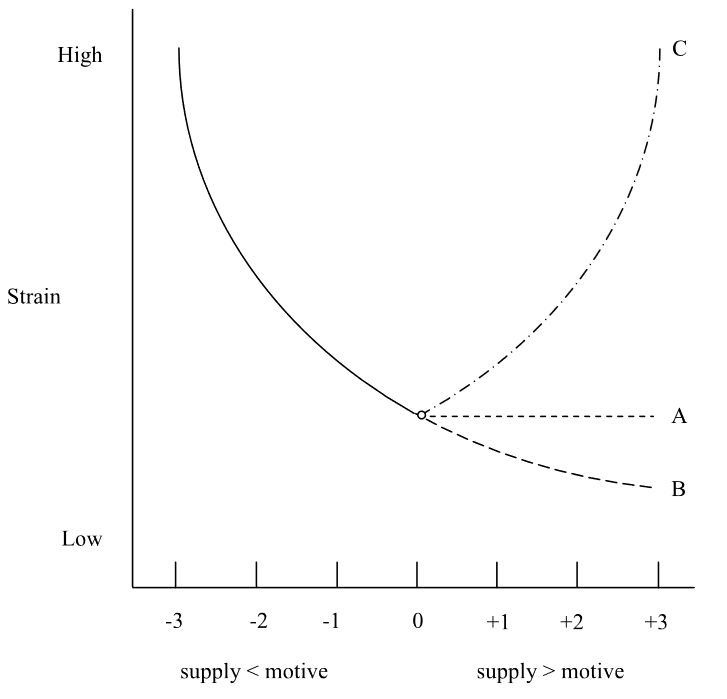
\includegraphics[width=0.75\textwidth]{gfx/ueberschuss_supply_motive.png}
	\caption{Hier eine Beschreibung einfügen \cite[S. 23]{edwards:2008}}
	\label{fig:personEnvironmentFit:auswirkungenErhoehterAngebote:abb1}
\end{figure}\\
An der durchgezogenen Linie auf der linken Hälfte von Abbildung \ref{fig:personEnvironmentFit:auswirkungenErhoehterAngebote:abb1} ist zu erkennen, dass je weniger die Bedürfnisse einer Person erfüllt werden, die mentale Belastung (Strain) des Individuums stärker zunimmt \cite{mechanismsOfJobStressAndStrain:1982}. Der Verlauf der linken Kurve kann über folgende algebraische Differenzberechnung bestimmt werden:
\begin{equation}
	B = P - E
	\label{fig:personEnvironmentFit:auswirkungenErhoehterAngebote:formel1}
\end{equation}
In Gleichung \ref{fig:personEnvironmentFit:auswirkungenErhoehterAngebote:formel1} steht $B$ für die mentale Belastung des Mitarbeiters. $P$ stellt die von einer Person gewünschte Menge eines bestimmten Wertes dar. Die vom Mitarbeiter wahrgenommene erhaltene Menge des entsprechenden Wertes seitens der Umgebung wird über Parameter $E$ ausgedrückt \cite[S. 2]{edwards:1993}.\\
Übersteigen die Angebote der Umgebung dagegen die Bedürfnisse der Person, mündet dies in einer der drei gepunkteten Linien A, B oder C.\\
Kurve A zeigt einen monotonen Verlauf der mentalen Belastung. Dieser entsteht, wenn eine Person die Übererfüllung eines Bedürfnisses entweder für einen späteren Zeitpunkt aufsparen oder in die Befriedigung verwandter Motive investieren kann \cite{mechanismsOfJobStressAndStrain:1982}. Dieser Sachverhalt ist beispielsweise erfüllt, wenn einer Person mehr Gehalt zusteht, als diese für die Zahlung ihrer Lebenskosten benötigt. Das überschüssige Geld könnte diese entweder für die Zahlung von Lebenshaltungskosten in den Folgemonaten aufsparen oder zusätzlich ihr mögliches Bedürfnis nach Luxusgütern befriedigen \cite[S. 21]{edwards:2008}. Für die Berechnung von Kurve A kann Gleichung \ref{fig:personEnvironmentFit:auswirkungenErhoehterAngebote:formel1} verwendet werden \cite[S. 2]{edwards:1993}.\\
Linie B hat den Verlauf einer quadratischen Funktion und tritt ein, wenn die Übererfüllung eines Bedürfnisses entweder die Befriedigung dieses oder eines verwandten Motivs hemmt \cite[S. 5]{caplan:1987}. \textcite{harrison:1978} nennt hierfür das Bedürfnis einer Person nach sozialem Austausch als Beispiel, welches bei Übererfüllung das Verlangen nach Privatsphäre verletzt. Der Verlauf von Kurve B kann über die in Gleichung \ref{fig:personEnvironmentFit:auswirkungenErhoehterAngebote:formel2} dargestellte algebraische Differenz bestimmt werden \cite[S. 2]{edwards:1993}.
\begin{equation}
	B = |P - E|
	\label{fig:personEnvironmentFit:auswirkungenErhoehterAngebote:formel2}
\end{equation}
Alternativ kann die quadrierten Differenzberechnung aus Gleichung \ref{fig:personEnvironmentFit:auswirkungenErhoehterAngebote:formel3} verwendet werden \cite[S. 2]{edwards:1993}.
\begin{equation}
	B = (P - E)^2
	\label{fig:personEnvironmentFit:auswirkungenErhoehterAngebote:formel3}
\end{equation}
Kurve C stellt eine asymptotische Beziehung zur mentalen Belastung dar. Sie tritt ein, wenn weder die Bedingungen von Kurve A noch von Linie B zutreffen. Eine Übererfüllung dieses Bedürfnisses hat folglich weder positive noch negative Folgen für die Person \cite{mechanismsOfJobStressAndStrain:1982}. Ein Beispiel für eine solche Beziehung ist ein Überangebot an Parkplätzen beim Arbeitgeber. Da der Mitarbeiter nur ein Fahrzeug besitzt, kann dieser von zusätzlichen Angeboten keinen Gebrauch machen und diese auch nicht für einen späteren Zeitpunkt aufsparen. Die zusätzlichen Parkplätze schaden auch keinem anderen Bedürfnis des Mitarbeiters. Somit entstehen weder positive noch negative Auswirkungen auf dessen Wohlbefinden. Zur Bestimmung von Kurve C wird die Belastung wie in Gleichung \ref{fig:personEnvironmentFit:auswirkungenErhoehterAngebote:formel4} dargestellt, gleich dem Wert null gesetzt \cite[S. 2]{edwards:1993}.
\begin{equation}
	B = 0
	\label{fig:personEnvironmentFit:auswirkungenErhoehterAngebote:formel4}
\end{equation}
Verschiedene Autoren gehen davon aus, dass die Beziehungen aus Abbildung \ref{fig:personEnvironmentFit:auswirkungenErhoehterAngebote:abb1} auch für den Anforderungen-Fähigkeiten Fit zu erwarten sind. Dies gilt wie in Kapitel \ref{ch:personEnvironmentFit:subjektivObjektiv} beschrieben nur, wenn das Erfüllen der Anforderungen Auswirkungen auf die inneren Werte des Mitarbeiters hat \cite{mechanismsOfJobStressAndStrain:1982, harrison:1978}. Wie an der durchgezogenen Linie in Abbildung \ref{fig:personEnvironmentFit:auswirkungenErhoehterAngebote:abb1} zu erkennen, entsteht psychische Belastung, wenn die Anforderungen der Umgebung die Kenntnisse des Mitarbeiters übersteigen \cite[S. 5]{schuler:1980}. Sind dagegen die Fähigkeiten des Angestellten stärker ausgeprägt als erforderlich, resultiert eine der Kurven A bis C. Linie A tritt ein, wenn der Mitarbeiter seine gewonnenen Freiräume nutzen kann, um verwandte Bedürfnisse zu erfüllen. Schaden die zu niedrigen Anforderungen einem Bedürfnis des Mitarbeiters, entsteht Kurve B. Haben die zu hohen Fähigkeiten des Angestellten weder positive noch negative Auswirkungen auf dessen Wohlbefinden, resultiert Linie C \cite[S. 22f.]{edwards:2008}.\\
Unterschiedliche Publikationen stellen fest, dass der Verlauf der Kurven nicht alleine von den Auswirkungen der Misfits auf die Motive des Mitarbeiters abhängig ist. Zusätzlich muss beachtet werden, als wie wichtig der Angestellte die betroffenen Bedürfnisse bewertet \cite[S. 9f.]{edwards:1996}. 

\section{Einbeziehung der Wichtigkeiten von Bedürfnissen}
\label{ch:personEnvironmentFit:wichtigkeiten}
Bereits bei der ersten formalen Vorstellung des Person-Environment Fits empfahlen \textcite{copingAndAdaption:1974} die Einbeziehung von Wichtigkeitswerten in die Berechnung. Auf welche Weise diese Werte einbezogen werden sollten, ließen die Autoren zum damaligen Zeitpunkt jedoch unbeantwortet \cite[S. 19]{edwards:2008}.\\
\textcite[S. 38]{harrison:1985} schlug später vor, den P-E Fit für jede untersuchte Variable einzeln zu berechnen und mit einem subjektiven Wichtigkeitswert zu multiplizieren. Diese Einschätzung teilte auch \textcite[S. 18]{locke:1969}\cite[S. 8f.]{locke:1976}. Er gilt als einer der einflussreichsten Wissenschaftler auf dem Gebiet der Arbeitszufriedenheit \cite[S. 12]{edwards:2008}. Diese kann laut \textcite[S. 8]{locke:1969} nur entstehen, wenn Mitarbeiter das Gefühl haben, für sie als wichtig erachtete Werte durch ihre Tätigkeit zu erfüllen. Aus diesem Grund empfahl er zur Berechnung der Arbeitszufriedenheit eines Angestellten zwei Kennzahlen heranzuziehen: Die Differenz aus wahrgenommener und gewünschter Menge eines Wertes und die subjektive Wichtigkeit des Motivs \cite[S. 8]{locke:1976}. \textcite[S. 16]{locke:1969} betonte, dass je nach untersuchtem Wert unterschiedliche Subtraktionen wie algebraische oder absolute Differenz durchgeführt werden können. Ein Beispiel für eine Berechnung mit algebraischer Differenz ist in folgender Gleichung \ref{fig:personEnvironmentFit:wichtigkeiten:formel1} dargestellt (vgl. \cite[S. 9]{edwards:1990}):
\begin{equation}
	Y = b * (P - E)
	\label{fig:personEnvironmentFit:wichtigkeiten:formel1}
\end{equation}
In Gleichung \ref{fig:personEnvironmentFit:wichtigkeiten:formel1} steht $Y$ für das untersuchte Ergebnis, wie beispielsweise die Arbeitszufriedenheit. $b$ stellt den subjektiven Wichtigkeitswert dar. Dieser wird mit der Differenz aus gewünschte Menge eines Wertes einer Person $P$ und wahrgenommener Menge des Wertes der Umgebung $E$ multipliziert (vgl. \cite[S. 9f.]{edwards:1990}).\\
Derartige Multiplikationen mit einem Differenzwert haben zur Folge, dass die in Abbildung \ref{fig:personEnvironmentFit:auswirkungenErhoehterAngebote:abb1} dargestellten Kurven mit steigender Wichtigkeit steiler werden \cite[S. 9]{locke:1976}. Abbildung \ref{fig:personEnvironmentFit:wichtigkeiten:abb1} verdeutlicht solche Stauchungen durch Wichtigkeitswerte.\\
\begin{figure}[h]
	\centering
	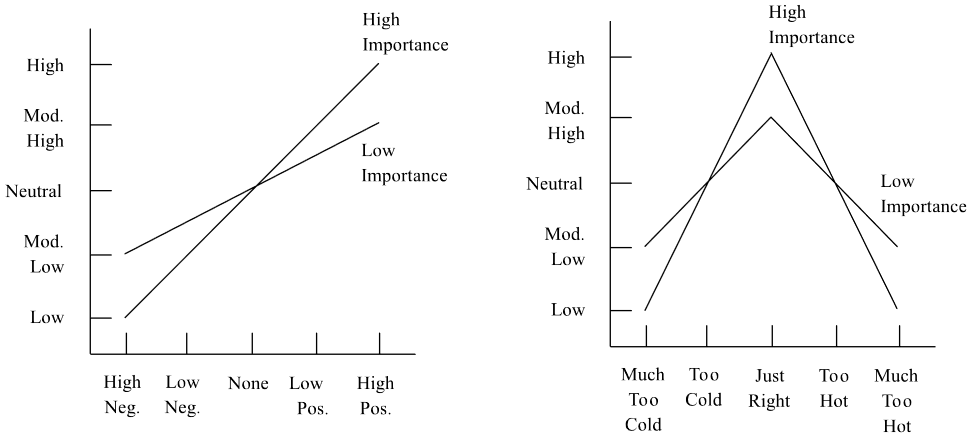
\includegraphics[width=1\textwidth]{gfx/Locke.png}
	\caption{Stauchung von Funktionsgraphen durch Wichtigkeitswerte (Aus \cite[S. 13f.]{edwards:2008}, nach \cite[S. 1305]{locke:1976})}
	\label{fig:personEnvironmentFit:wichtigkeiten:abb1}
\end{figure}\\
\textcite[S. 51ff.]{edwards:1991}\cite[S. 9ff.]{edwards:1990} kritisierte Berechnungen wie in Gleichung \ref{fig:personEnvironmentFit:wichtigkeiten:formel1} in mehreren seiner Arbeiten. Dabei diskutierte er insbesondere die Multiplikation mit dem Differenzwert. Edwards ist der Auffassung, dass die aus der Differenzberechnung resultierenden zweidimensionalen Grafiken die Komplexität eines P-E Fits nicht vollständig abbilden. Deshalb empfahl er, gewünschte und wahrgenommene Menge nicht als einen Index, sondern als separate Kennzahlen zu multiplizieren. Formel \ref{fig:personEnvironmentFit:wichtigkeiten:formel1} könnte dazu folgendermaßen umgestellt werden:
\begin{equation}
	Y = b_1 * P - b_2 * E
	\label{fig:personEnvironmentFit:wichtigkeiten:formel2}
\end{equation}
$b_1$ und $b_2$ stehen in Gleichung \ref{fig:personEnvironmentFit:wichtigkeiten:formel2} für die separaten Wichtigkeiten von gewünschter $P$ und wahrgenommener Menge $E$ eines Wertes. Durch diese Art der Berechnung entstehen laut Edwards aus zweidimensionalen Grafiken dreidimensionale Modelle. Solche Darstellungen sind dem Wissenschaftler zu Folge besser geeignet, Ungleichmäßigkeiten in den Oberflächen darzustellen. So stellte \textcite[S. 53ff.]{edwards:1991} bei der Datenanalyse einer Studie mit mehreren hundert Teilnehmern die in Abbildung \ref{fig:personEnvironmentFit:wichtigkeiten:abb2} dargestellte dreidimensionale Beziehung von P-E Fit und Zufriedenheit fest.\\
\begin{figure}[h]
	\centering
	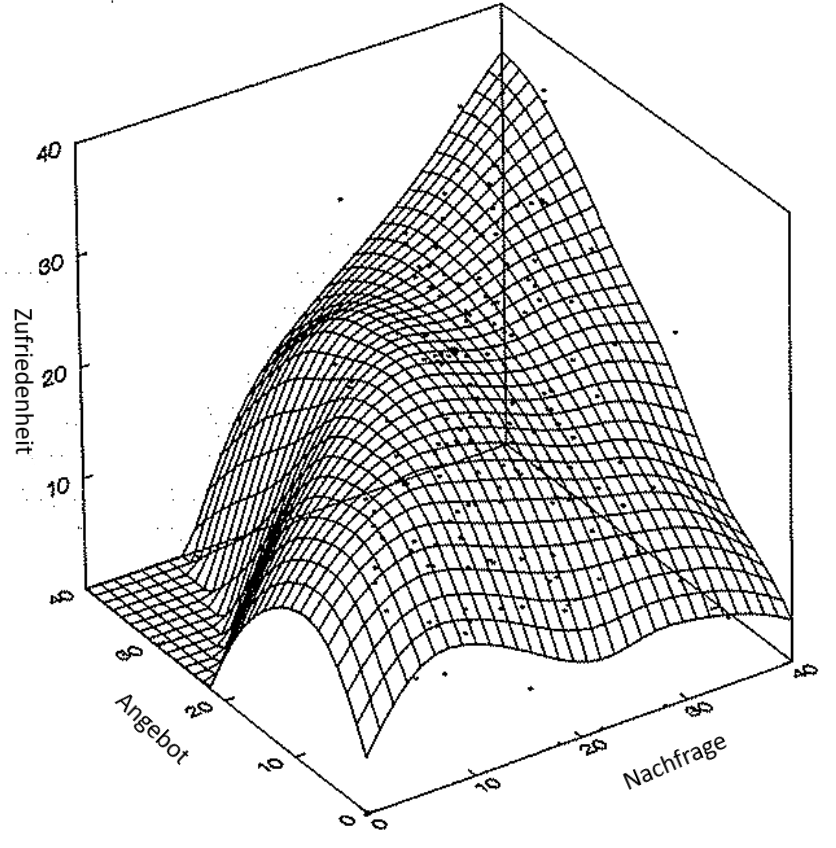
\includegraphics[width=0.75\textwidth]{gfx/drei_d_modell.png}
	\caption{Hier eine Beschreibung einfügen \cite[S. 57]{edwards:1991}}
	\label{fig:personEnvironmentFit:wichtigkeiten:abb2}
\end{figure}\\


\newpage
\section{Berechnung}
\label{ch:personEnvironmentFit:berechnung}
- \cite[S. 15f.]{caplan:1993}: Edwards schlägt eine generelle Prozudur vor, die es erlaubt die Eignung von Bedingungen und Annahmen zu bestimmen --> Prozedur erlaubt die Beziehung zwischen outcome und Kongruenz auf drei Dimensionen (Bild-->zu sehen sind die Rohdaten von Caplan et al 1980) --> Dabei ist die abhängige Variable vertikal / \cite[S. 16]{caplan:1993}: Ansatz von Edwards: Statt einen Differenz-Wert zu berechnen, nimmt man die Regressionsgleichung der Modelle (z.B. von absoluter oder algebraischer Differenz) --> Dann bestimmt man Anteil der erklärten Varianz (??)\\
- \cite[S. 2]{edwards:1993}: Es gibt viele Probleme an den 5 Messungen von Caplan und French (Quellen) --> Liegt an der Verwendung von Differenz-Berechnungen --> Es folgt Kritik dazu --> Probelme mit den fit Messungen können durch andere von Edwards beschriebenen Prozeduren überwunden werden --> Edwards führt in diesem Paper die Forschungen von French et al 1982 erneut aus und wendet seine empfohlenen Berechnungen darauf an --> \cite[S. 19]{edwards:1993}: Ergebnisse: 1. fit Messungen, die E und P in einen Wert zusammenrechnen sollten zugunsten von Polyomialgleichungen, welche E und P und geeignete Terme höherer Ordnung enthalten, aufgegeben werden (Quellen) / Edwards Studie demonstrierte, dass fit Messungen zu mehrdeutigen Ergebnissen führen, die separaten Beziehungen von E und P mit strain durcheinander bringen, einen sehr restriktiven Satz von Beschränkungen auferlegen, die selten unterstützt werden und reduzieren die inhärente dreidimensionale Beziehung zwischen E, P und strain auf zwei Dimensionen / \cite[S. 20]{edwards:1993}: Edwards (Quelle) Prozedur vermied diese Probleme und zeigte in den meisten Fällen, dass die Beziehung zwischen E, P und strain konnte nicht adäquat von den fit Messungen von French et al 1982 repräsentiert werden --> Grund: Diese Prozedur nutze Gleichungen, welche Fit-Messungen subsummieren, dies eliminierte die Notwendigkeit für diese Messungen und erlaubte darüber hinaus die Mesung von einer breiteren Rand von Oberflächen bezogen auf E und P zu strain --> Weitere Punkte (nachlesen)\\
- \cite[S. 7]{su:2015}: Verwendung von fit-Indizes ist wegen der Einfachheit des Kongruenzwertesn sehr beliebt in der Karriere-Entwicklungsforschung --> Kritisiert von Edwards --> Alternativer Ansatz von Edwards (1994, 2002): Nutzung von polynominaler Regression --> Basiert auf der Prämisse, dass P und E Messungen verschiedene Konstrukte sind und dass die funktionale Form sollte eher empirisch getestet werden als ein fit-Index angenommen zu werden; Laut Edwards sind die Gleichungen generalisierte Formen des fit-Indexes ohne ungewollte Annahmen über die Koeffizienten der Komponenten; Mit diesem Ansatz hat Edwards den Datensatz von French, Caplan und Harrison (1982) erneut analysiert und zeigte, dass er den Anteil erklärter Varianz mehr als verdoppeln konnte \\
- In \textcite{edwards:1991} werden sehr viele Methoden zur Verrechnung genannt \\

\section{Perfekter Fit}
\label{ch:personEnvironmentFit:perfekterFit}
- \cite[S. 4]{edwards:2004}: Kristof 1996, S. 6 stellt fest: "Der optimale P-O fit ist erreicht, wenn jeder Need einer Entität ist erfüllt durch einen anderen und sie teilen dieselben grundlegenden Charakteristiken" \\
- \cite[S. 23]{edwards:2008}: Es gibt auch Erweiterungen des Frameworks, die Minima an anderen Punkten als dem P-E fit haben --> Caplan 1983 S. 39 sagt z.B. dass der meist emotional zufriedenstellenste Punkt so liegt, dass er eine kleine Herausforderung generiert. / Es gibt noch weitere Erweiterungen, z.B. wie Vergangenheit und Zukunft den Fit beeinflussen könnten \\
- \cite[S. 6]{caplan:1987}: Dass der Tiefpunkt nicht bei P=E liegt, wurde bei Kobasa\&Puccetti 1983 diskutiert)

\section{Content von P und E Dimensionen}
\label{ch:notizen:contentVonPundEDimensionen}
- \cite[S. 6]{edwards:2007}: Dimensionen können auf einem Kontinuum von Generell bis speziell reichen --> Edwards schlägt drei Punkte vor: Global-, Domäne-, Facettenlevel der P und E Dimensionen / Beim globalen Level werden den Ähnlichkeiten als Ganzes ohne Bezug auf andere Vergleichsdimensionen miteinander verglichen --> beim Supplementary Fit genutzt --> z.B. um P und E oder P und andere P zu vergleichen (Quellen) / \cite[S. 7]{edwards:2007}: Domain-Level  isoliert breite Bereiche, aber unterscheidet keine Dimensionen innerhalb des Bereichs --> z.B. Werte, Persönlichkeit (Quellen) / Beim Facetten-Level wird die Ähnlichkeit spezifischer Dimensionen inerhalb breiter Bereiche verglichen, z.B. wenn man die demographische Ähnlichkeit nach Alter, Geschlecht, Rasse und Erziehung bestimmen will (Quellen) --> Gutes Bild dazu auf S. 10 \\

\section{Job Stress}
\label{ch:notizen:jobStress}
\subsection{McGrath}
\label{ch:notizen:jobStress:mcgrath}
- \cite[S. 6]{edwards:2008}: Manche Studien identifizieren Grenzen, die Bedingungen etablieren, unter denen P-E fit-Beziehungen auftreten sollten --> Dies Bedingungen werden als Moderatoren bezeichnet, die die Form oder Stärke der P-E fit Beziehung beeifnlussen --> Beispiel: Der Effekt von D-A wird stärker, wenn das Nichterfüllen der Anforderungen wichtige Konsequenzen hat (2 Quellen von McGrath)\\
- \cite[S. 2f.]{edwards:1990}: Der D-A fit erscheint in McGraths Stressmodell (Quelle nicht gefunden) --> Besagt, dass Stress durch Anforderungen des Umfeldes entstehen, welche die Fähigkeiten und Ressourcen einer Person übersteigen \\
- \cite[S. 16]{edwards:2008}: Konzept des P-E fit ist weit verbreitet in den Theorien des Job Stresses (Quellen); Manche Theorien fokussieren den N-S fit (Quellen), andere den D-A fit (Quellen) und andere beide gleichzeitig (\cite{mechanismsOfJobStressAndStrain:1982}) \\
- \cite[S. 16]{edwards:2008}: McGraths Modell von Stress und Performance: McGrath (Quellen) fokussiert den D-A fit. Laut McGrath (Quelle) entsteht Stress durch ein Ungleichgewicht zwischen Anforderungen des Umfeldes und den entsprechenden Fähigkeiten --> Existiert nicht objektiv, sondern wie es von der Person wahrgenommen wird; Um Stress wahrzunehmen muss er Person das Ungleichgewicht bewusst sein / Stress kann sowohl bei einer Über- als auch einer Unterbelastung entstehen / Stress tritt nur auf, wenn die Person glaubt, dass die Konsequenzen des nicht erreichens der Anforderungen wichtig sind / Stress ist ein D-A Misfit, der zunimmt umso größer die Abweichung ist / McGrath stellte die folgende Formel auf (Quelle):

\begin{equation}
	ES = C(|D-A|)
	\label{fig:formel2}
\end{equation}

- \cite[S. 16]{edwards:2008}: ES ist der erfahrene Stress (experienced stress); C sind die wahrgenommenen Konsequenzen (Consequences); D sind die wahrgenommenen Anforderungen (Demands) und A sind die wahrgenommenen Fähigkeiten (Abilities) / \cite[S. 17]{edwards:2008}: In einer Studie operationalisierte McGrath Stress als eine physikalische Erregung und fand heraus, dass diese hoch war, wenn die Differenz zwischen Anforderungen und Fähigkeiten klein war (Quelle) --> McGrath interpretierte dieses Ergebnis als ein Manifestierung von Unsicherheit basierend auf der Annahme, dass die Unsicherheit eine Aufgabe zu erfüllen zunimmt, wenn die Anforderungen und Fähigkeiten nah beieinander sind --> Annahme: Erfolg wird wahrscheinlich, wenn Fähigkeiten die Anforderungen übersteigen und Verlust wird wahrscheinlich, wenn die Anforderungen die Fähigkeiten übersteigen --> Aus dieser Schlussfolgerung passte McGrath seine Formel an:

\begin{equation}
	ES = C(K-|D-A|)
	\label{fig:formel3}
\end{equation}

- \cite[S. 17]{edwards:2008}: K ist dabei eine Konstante --> Dadurch dass |D-A| von K abgezogen wird, zeigt die Gleichung, dass Stress (bzw. Erregung) zunimmt, wenn die Lücke zwischen D und A abnimmt \\
- \cite[S. 18]{edwards:2008}: Die Definition von Stress als Erregung wird in der Stress-Literatur diskutiert (Quellen)

\section{Berufliche Kongruenz}
\label{ch:notizen:beruflicheKongruenz}
\subsection{Dawis und Lofquist}
\label{ch:notizen:beruflicheKongruenz:dawisUndLofquist}
- \cite[S. 31]{edwards:2008}: Die letzte Version (Dawis und Lofquist 1984) definiert Fähigkeiten als empirisch abgeleitete Faktoren, die spezifische Fähigkeiten umfassen, die "wiederkehrende Reaktionssequenzen sind, die dazu neigen, durch Wiederholung modifiziert und verfeinert zu werden" (Zitat) / Analog dazu sind Values Faktoren, die spezifische Needs umfassen, die definiert sind als "Das Bedürfnis eines Individuums nach einem Verstärker auf einem bestimmten Niveau der Stärke" --> Stärke ist die Wichtigkeit eines Bedürfnisses --> Ich schließe aus dem Kontext: Je größer die Stärke, desto Häufiger muss die Reaktion des Verstärkers sein; Werte sind Wichtigkeitsdimensionen als Referenzdimensionen für die Beschreibung von Needs --> Needs sind Präferenzen für Verstärker ausgedrückt als relative Wichtigkeit für jeden Verstärker für das Individuum / Definition Korrespondenz: "Harmonische Beziehung zwischen Individuum und Umgebung, Eignung des Individuums für die Umwelt und der Umwelt für das Individuum, Übereinstimmung oder Einvernehmen zwischen Individuum und Umgebung sowie eine wechselseitige und ergänzende Beziehung zwischen Individuum und Umwelt" --> Es besteht also eine wechselseitige Beziehung zwischen Individuum und Umgebung / Definitionen für Zufriedenheit und Zufriedenstellung \\

\section{Recruiting und Selektion}
\label{ch:notizen:rekcruitingUndSelektion}
- \cite[S. 33]{edwards:2008}: P-E fit ist fundamental, wenn Menschen mit Jobs in Unternehmen gematcht werden (Quellen) / Forschung in diesem Bereich identifiziert meist das notwendige Wissen, Fertigkeiten und Fähigkeiten für einen Job, misst diese Attribute bei möglichen Angestellten und untersuchen den Zusammenhang zwischen diesen Messungen und späterer Arbeitsleistung (Performance) --> Diese Forschung adressiert nicht direkt den Fit zwischen Person und Job, weil die persönlichen Attribute nicht berücksichtigt werden (Schneider, 2001) --> Edwards betrachtet nur Theorien, die explizit den P-E fit behandeln
- \cite[S. 5]{su:2015}: Werbel und Gilliland 1999 erstellten einen multilevel Ansatz, welcher den Selektionsprozess in Bezug auf P-J, P-O und P-G abbildet; P-J ist definiert als die Kongruenz zwischen Demands des Jobs und Skills, Knowledge und Abiligies des Job Kandidaten und soll vorhersagen den Leistungsstand des Kandidaten, sein technisches Verständnis und die Arbeitsinnovation; P-O bezieht sich auf die Kompatibilität zwischen den Needs, Zielen und Values des Bewerbers mit den Normen, Werten und Belohnungssystemen der Organisation und sagt voraus das Verhalten, Commitment und Zurückhaltung; P-G fit stellt die Ähnlichkeit zwischen einer Person und den Mitgliedern einer Arbeitsgruppe in Bezug auf deren Werte, Ziele, Persönlichkeit, etc. fest --> sagt voraus Kooperation und Performance \\

\subsection{Breaughs Person-Job Congruence Model}
\label{ch:notizen:rekcruitingUndSelektion:breaugh}
- \cite[S. 36]{edwards:2008}: Braugh entwickelte ein Modell für einen Rekruting-Prozess der die person-job Kongruenz als zentrale Komponente unterstützt --> P-J Kongruenz definiert er als "Diskrepanz zwischen den Attributen, die ein e Organisation von einem potentiellen Angestellten verlangt und den Charakteristiken die eine Person bietet und die Diskrepanz zwischen dem was die Person von der Organisation will und den Anreizen, die der Arbeitgeber bietet" --> \cite[S. 37]{edwards:2008}: (Zitate) D-A fit führt zu einem zufriedenstellenden Level an Job-Performance und ein guter fit zwischen den Wünschen der Person und den Attributen der Job-Angebote führt zu einem Gefühl der Wertsteigerung, was wiederum zu Arbeitszufriedenheit führen wird" / Nachteil nach Edwards: Beschreibt keine Metrik, mit der Person und Job verglichen werden können --> Aber es gibt ein paar Beispiele / In einer Fußnote schreibt Breaugh, dass der P-J fit sich auf die Wahrnehmung der Kongruenz zw. DA und SV bezieht (das muss ich nochmal nachprüfen) / Modell bleibt auch wage bei der Form der Beziehung zwischen Kongruenz udn Outcomes --> In einer Fußnote stellt Breaugh fest, dass für manche Organisationalen Attribute ein Individuum weder zu viel noch zu wenig von einem Attribut sucht (z.B. Reisen). Bei anderen Attributen gitl, umso mehr die Organisation bietet (z.B. Bezahlung) desto besser wird die Person den fit bewerten --> Bestimmte Attribute werden aber nicht genannt

\subsection{Werbel and Gillilands Facet Model of Fit}
\label{ch:notizen:rekcruitingUndSelektion:werbel}
- \cite[S. 37]{edwards:2008}: Werbel und Gilliland stelleten ein Faketten-Modell des P-E fits vor, welches den Auswahlprozess in Bezug auf Person-Job fit, Person-Workgroup fit und Person-Organization fit bezieht / P-J fit ist definiert als (Zitat) Kongruenz zwischen Job-Anforderungen und den benötigten Skills, Wissen und Fähigkeiten eines Job-Kandidaten --> \cite[S. 38]{edwards:2008}: Laut 
Modell führt der P-J fit zu Leistung, technischem Verständnis und Arbeitsinnovationen / Person-Workgroup fit bezieht sich auf das (Zitat) Match zwischen dem Neuangestellten und der gesamten Arbeitsgruppe (z.B. Mitarbeiter und Führungskräfte) --> P-W fit wird sowohl durch einen supplementary als auch einen complementary fit bestimmt: Supplementary, da Werte, Ziele, Persönlichkeit übereinstimmen müssen und complementary, da die Gruppe heterogene Skills, Leistungen und Netzwerke mitbringen muss, sodass (Zitat) Performance-Schwächen eines Individuums durch die Performance-Stärken eines anderen Individuums ausgeglichen werden können / P-O fit enthält einen supplementary fit und einen needs-supply fit; Supplementary fit ist beschrieben als Kompatibilität zw. dem Wertesystem der Person und der Organisation; NS fit bezieht sich auf das Match (Zitat) zwischen den Bedürfnissen des Bewerbers und dem organisationalen Belohnungssystem --> Ergebnis des Fits sind Organizational Citizenship Behaviors (OCBs), organisationale Zufriedenheit, organisationales Commitment und Bewahrung / Die Outcomes aller drei fits sind mit insgesamter Performance und organisationaler Effektivität verbunden / Kommentare von Edwards: Modell ist dahingehend bemerkenswert, dass es drei Typen von P-E Fits betrachtet und kollektiv NS und DA und supplementary fit anspricht\\
- \cite[S. 3]{edwards:1990}: Der D-A fit unterliegt laut Schneider 1978 und Smith und Robertson 1989 (noch nicht nach Quellen recherchiert) dem am verbreitetsten Personalauswahl-Modell --> Job Anforderungen analysieren, benötigte Fähigkeiten definieren und Personen anstellen, die diese Fähigkeiten beherrschen (Anmerkung von mir: Genauso arbeiten heute auch die meisten Recommender Systeme) \\

\section{ToDo}
\label{ch:todo}
- \cite[S. 2]{edwards:2008}: Meta-Analysen (Quellen)\\
- Manche Arbeiten unterscheiden zwar explizit zwischen subjektiven und objektiven P und E --> Ausnahme von der Regel (Edwards) --> bei SV-fit ist subjektive Wahrnehmung üblich \\
- Am Anfang Edwards Definitionen für P, E, fit und P-E fit verwenden, danach einzelne Definitionen für die Konstrukte suchen \\
- Was ist organisationales Verhalten \\
- Gliederung: Wichtigkeiten und dann sagen, dass aber auch Autoren zum Ergebnis kommen, dass DA für Individuum vollkommen egal ist --> Reinforcers --> Obwohl diese Verstärker so wichtig sind, werden sie bei der Personal-Auswahl häufig vernachlässigt (nur DA) --> Diese fehlende Beachtung von SV spiegelt sich auch in der Implementierung von Empfehlungssystemen wieder --> Switch zu RS \\
- Merke ein Konstrukt ist z.B. Demand oder Supply \\
- Es ist nicht möglich, alle Varianten und Arbeiten zu behandeln, wie geht man damit um? \\
- Interessant: Supplies werden auch als "Verstärker" für Needs betrachtet \\
- Nochmal nach den Definitionen für DA und SV bei Edwards suchen \\
- Es gibt viele Arten von Fits (PO, PJ, PW, etc.) --> Klar machen, dass hier nur PJ fokussiert wird (PW siehe Werbel; PO siehe O-Klima bzw. Schneider bei Klima) \\
- Wichtigkeit spielt vor allem beim supplementary fit eine Rolle --> Dieser wird in dieser Arbeit eher ausgeklammert, weil ich mich auf P-J fokussiere und supplementary eher verwendet wird, um zu schauen ob eine Person zu anderen Personen oder überhaupt in eine Org passt. Dennoch spielen Wichtigkeiten auch in manchen Umsetzungen des complementary fit eine Rolle. --> Wichtigkeiten \\
- Wichtigkeiten beziehen sich bei SV auf die Werte bei DA auf die Konsequenzen --> Person ist es egal, ob sie Anforderungen erfüllt --> Neues Kapitel \\
- Eigentlich ist es mir als Person nur wichtig meine eigenen Werte zu erfüllen (SV) --> D.h. "Performance" ist nur ein Nebenergebnis der SV-Erfüllung \\
- Lazarus nochmal prüfen \\
- - \cite[S. 8]{caplan:1987}: Der erste reale Test der PE fit Theorie unter Verwendung vergleichbarer Messungen von P und E erschien in Pervin 1967a und 1967b in einer Studie der Adaption unter Universitäts-Studenten --> Schlechter Fit zwischen Menge an Struktur im Bildungsansatz der Universität und dem Bedürfnis des Studenten nach Struktur wurde mit akademischer Unzufriedenheit und einem Studienabbruch aus nicht-akademischen Gründen assoziiert --> Seit Pervins Foschung sind viele Tests zur PE fit Theorie durchgeführt worden (zahlreiche Quellen) --> In diesen nachfolgenden Arbeiten ist mit wenigen Ausnahmen zu beobachten, dass einander entsprechend gemessene P und E signifikant zur erklärten Varianz beitrugen, die über die erklärte Varianz durch P oder E alleine hinausgeht\\

\section{Fazit}
\label{ch:fazit}
- Ob man die Anforderungen der Stelle erfüllt, ist dem Mitarbeiter eigentlich egal. Ihn interessiert es nur, ob dadurch seine Werte verstärkt/erfüllt werden. Es wäre also interessant, herauszufinden, wieso ein Mitarbeiter z.B. mehr Python anwenden würde. Mehr Gehalt wegen Data Science? Neugier für neue Sprache? Kumpel arbeitet in dieser Abteilung? ... \\
- Eigentlich müsste der Prozess des Motivations-Herausfindens dem kompletten Einstellungsprozess vorgelagert sein. Bzw. sogar dem Studium \\
- Grenze: \textcite{cable:1997} stellten fest, dass das Bauchgefühl des Interviewers besser vorhersagen kann, ob eine P zur O passt. Wenn also ein Unternehmen so klein ist, dass der "Staffer" alle Berater persönlich kennt, kann er wahrscheinlich besser zuordnen als die KI \\
- Anmerkung von mir: Während \textcite{parsons:1909} 1909 also noch davon ausging, dass alles möglichst objektiv und wissenschaftlich korrekt gemessen werden muss, gehen Psychologen heute davon aus, dass primär die subjektive Wahrnehmung eine Hauptrolle spielt \\

\section{Fragen}
\label{ch:fragen}
- Die historischen Bücher sprechen immer nur von "Männern" --> kann man daraus einfach "Menschen" machen?\\
- Gründungsvater ist ein englisches Zitat --> Wie zitieren?\\
- Wie umgehen mit den englischen Begriffen? z.B. fit, Need, Desire, etc.

%- \cite[S. 4]{su:2015}: Außerdem formulierte Chatman einen Sozialisationsprozess, durch welchen die Organisation seine Mitglieder beeinflusst, deren persönliche Werte in Einklang mit den Werten der Organisation zu bringen / Outcomes des PO-fits inkludieren Änderungen von persönlichen und Organisationalen Werten in Richtung eines erhöhten P-O fits / Individuen, die einen höheren Fit mit ihrer Organisation erreichen, kann zu positiven Karriere-Outcomes führen, inkl. erhöhten Betriebszugehörigkeit, Zufriedenheit, Commitment, Kompetenz, etc. / Auch Chatman stellt fest, dass ein sehr hohes Level an fit zu ineffektivem Verhalten auf Seiten von Individuum und Organisation führen kann --> Äußert sich z.B. in reduzierter Innovation \\
%- \cite[S. 11f.]{su:2015}: Bei Dawis and Lofquist 1976 und 1978 bezieht sich die Korrespondenz nicht auf einen statischen Zustand, sondern eher auf einen Prozess der "corresponsiveness", in welchem P und E gegenseitig aufeinander reagieren --> Änderungen am Fit treten auf, wenn sich bei P und E aufeinander anpassen, um einen besseren Fit zu erzielen --> Zu diesem Ergebnis kommt auch Roberts 2006, dieser erweiterte Schneiders ASA Framework zu ASTMA (Attraction, selection, transformation, maniplulation, attrition) bei P-O Transaktionen --> Hierbei besagt insbesondere Transformation, dass sich Menschen durch ihre Arbeitserfahrungen ändern können, so kann sich ihr objektiver oder wahrgenommener fit ändern; Manipulation bedeutet, dass nicht nur passiv die Demands von E erfüllen, sondern aktiv die Organisation ändern oder ihre eigene Arbeitserfahrung anpassen, um den fit zu maximieren \\
%- \cite[S. 1]{caplan:1987}: Ein einzigartiges Merkmal des Frameworks ist seine Operationalisierung: Bewertung von P und E  Komponenten entlang von vergleichbaren Dimensionen \\
%- \cite[S. 4]{caplan:1987}: Der Anpassungsgrad wird in der PE-Fit-Theorie als der Betrag der Verbesserung des PE-Fits im Laufe der Zeit definiert --> Anpassungsprozess bezieht sich darauf, wie Verbesserung (oder Verschlechterung) erreicht wird --> Wie in Fig 1 dargestellt, gibt es verschiedene Punkte der Intervention --> Einer kann sich auf objektive P und E beziehen; Einer kann sich auf den Versuch der Veränderung von den subjektiven Gegenstücken beziehen --> Im Text: Anpassung von objektiven und subjektiven P und E, z.B. durch Selektion oder Training \\
%- \cite[S. 4]{caplan:1987}: Wenn man darlegen kann, wie der P-E fit erreicht wurde, kann das Mitgliedern der Organisation helfen zu bestimmen, ob Selektion, Training, menschliche Faktoren oder andere Ansätze ihre gewollten Effekte erreicht haben\\
%- \cite[S. 1f.]{edwards:2007}: Die Forschung zum PE fit hat 3 grundlegende Annahmen: 1. Es wird generell angenommen, dass der PE fit zu positiven Outcomes führt (Quellen); 2. Es wird oft angenommen, dass die Auswirkungen des PE-Fits die selben über mehrere Personen- und Environments Konstruke sind (Quellen); 3. \cite[S. 2]{edwards:2007}: Effekte des PE fits sind die selben, unabhängig von den absoluten Levels von P und E oder der Richtung ihrer Differenz --> Quellen, die Ähnlichkeiten berechnen; Annahmen wurden diskutiert und in Frage gestellt, halten sie sich dennoch weitgehend in der PE Forschung\\
\shorthandon{"}